\documentclass[a4paper,12pt]{article}

\usepackage{amsfonts}
\usepackage{amsmath}
\usepackage{float}
\usepackage{graphicx}
\usepackage{listings}
\usepackage[margin=1in]{geometry}

\title{Assignment 3: Applications of Image Processing to Real-World Problems}
\author{Aleksandr Jan Smoliakov}
\date{2024--12--20}

\begin{document}

\maketitle

\section{Introduction}

As a final report in the trilogy, this document explores the practical applications of image processing techniques to real-world problems. It builds upon the theoretical foundation established in the previous assignments and demonstrates the application of these concepts to solve specific challenges in diverse domains.

The first section, \textbf{Theoretical Background}, provides an overview of the theoretical background, including concepts such as thresholding, morphological operations, and image segmentation.

The subsequent sections present three distinct applications of image processing techniques to real-world problems.

In \textbf{Application: FISH Signal Counts}, we analyze fluorescence in situ hybridization (FISH) images to detect and quantify genetic mutations in tumor cells. This involves identifying mutations using fluorescent probes and quantifying the signals to understand the mutation distribution within individual cells.

In \textbf{Application: Circuit Board Quality Assurance}, we analyze images of circuit boards to detect defects. This involves inspecting soldering regions, traces, and drilled holes using x-ray imaging and image processing techniques.

In \textbf{Application: Filled Bottles}, we analyze images of a production line to detect whether bottles are filled to the correct level. This involves detecting the liquid level in bottles using edge detection and intensity analysis.

\newpage

\tableofcontents

\newpage

\section{Theoretical Background}

Understanding the real-world applications described in the next sections of this report requires familiarity with several key concepts in digital image processing. This section provides a brief overview of these concepts.

\subsection{Colour Image Processing}

In digital images, colour is commonly represented by three components, denoted as \(R\), \(G\), and \(B\) for the red, green, and blue channels respectively. Each pixel \((x, y)\) in a colour image \(f\) can thus be expressed as:
\[
f(x, y) = \bigl(R(x, y),\, G(x, y),\, B(x, y)\bigr).
\]
Each channel captures intensity information for its respective colour. The range of each intensity value typically spans from 0 to 255 in 8-bit images, or can be extended for higher bit-depth images. Colour perception in imaging is based on an \emph{additive} mixture of these channels.

\subsubsection{Pseudo Colour Image Processing}

Pseudo colour (or false colour) image processing is a technique that maps intensity values of a grayscale image to a colour map. The goal is to improve the perception or interpretability of certain image structures. For instance, a temperature map might be converted to a spectrum ranging from blue (cool) to red (hot).

Mathematically, let \(I\) be a grayscale image with pixel intensities in the range \([0, 1]\). A pseudo colour function \(\Phi\) maps each intensity to a triplet of colour values:
\[
\Phi: [0,1] \rightarrow \mathbb{R}^3, \quad I(x,y) \mapsto (R, G, B).
\]

\subsubsection{Full Colour Image Processing}

Full colour image processing involves manipulating or analyzing images in their three-channel (or multi-channel) format. Typical tasks include:

\begin{itemize}
    \item \textbf{Colour Enhancement}: Adjusting brightness, contrast, or gamma in one or more channels to improve visual quality.
    \item \textbf{Colour Balancing}: Correcting or normalizing images, for example by imposing white balance to ensure a neutral background.
    \item \textbf{Segmentation and Object Recognition}: Using features in the colour space to isolate objects (e.g. detecting green plants against a darker background in an agricultural scene).
\end{itemize}

The general colour transformation in full colour image processing can be expressed as:
\[
\begin{bmatrix}
R' \\
G' \\
B'
\end{bmatrix}
=
\begin{bmatrix}
r_{11} & r_{12} & r_{13} \\
r_{21} & r_{22} & r_{23} \\
r_{31} & r_{32} & r_{33}
\end{bmatrix}
\begin{bmatrix}
R \\
G \\
B
\end{bmatrix}
+
\begin{bmatrix}
r_{10} \\
r_{20} \\
r_{30}
\end{bmatrix},
\]
where the matrix \([r_{ij}]\) and vector \([r_{i0}]\) represent the transformation coefficients.

\subsubsection{Noise in Colour Images}

Noise in colour images can arise from various sources such as sensor electronics or lighting conditions. Unlike grayscale images, where noise typically appears as isolated intensity fluctuations, noise in colour images can affect each channel differently - or not at all. Models of noise include:

\begin{itemize}
    \item \textbf{Additive Gaussian Noise (AGN)}: Often assumed in raw sensor data, where each channel \(c \in \{R, G, B\}\) is contaminated by independent Gaussian noise \(n_c\).
    \[
    c_{noisy}(x,y) = c_{true}(x,y) + n_c(x,y), \quad n_c \sim \mathcal{N}(0,\,\sigma^2).
    \]
    \item \textbf{Salt-and-Pepper Noise}: Prevalent in digital transmission errors or faulty pixels, leading to random instances of maximum or minimum intensity in each channel.
\end{itemize}

Denoising methods for colour images often extend grayscale techniques (e.g. median or Gaussian filters) to each channel separately or adopt vector-based approaches to better preserve chromatic relationships.

\subsection{Thresholding}

Thresholding is a fundamental technique in digital image analysis used to separate objects of interest from the background. The process assigns a binary label to each pixel based on a predefined intensity level called the \emph{threshold}. Mathematically, for a grayscale image \(f(x, y)\) and a threshold \(T\), the thresholded image \(g(x, y)\) can be expressed as:

\[
g(x, y) = 
\begin{cases}
1, & \text{if } f(x, y) \geq T, \\
0, & \text{otherwise}.
\end{cases}
\]

Here, \(g(x, y)\) is referred to as a \emph{binary} image, where \(1\) typically denotes foreground (e.g. object of interest) and \(0\) denotes background. Depending on the application, the foreground can represent different elements (e.g. cells in a microscopy image or elements in a circuit board).

This technique can be extended to \emph{multiple thresholding} where more than two classes are defined based on different intensity ranges. Mathematically, for \(n\) thresholds \(T_1, T_2, \ldots, T_n\), the thresholded image \(g(x, y)\) can be expressed as:

\[
g(x, y) =
\begin{cases}
1, & \text{if } f(x, y) \geq T_n, \\
\vdots & \\
n, & \text{if } T_{n-1} \leq f(x, y) < T_n, \\
0, & \text{otherwise}.
\end{cases}
\]

However, in the subsequent material, we focus on the basic binary thresholding technique for simplicity and clarity.

\subsubsection{Basic Global Thresholding}

The simplest form of thresholding assumes a single, constant threshold \(T\) that partitions the image into two classes (background and foreground). To determine this threshold, one can examine the intensity histogram of the image. A straightforward approach is to choose \(T\) as the \emph{midpoint} between the average foreground and average background intensities, or use domain-specific heuristics.

An improved version of basic global thresholding involves iterative selection:
\begin{enumerate}
    \item Select an initial estimate for the global threshold \(T\).
    \item Segment the image into background and foreground using \(T\).
    \item Compute the mean intensities \(\mu_b\) and \(\mu_f\) of the background and foreground classes, respectively.
    \item Update \(T \leftarrow \frac{\mu_b + \mu_f}{2}\).
    \item Repeat until \(T\) converges (i.e. the change \(\Delta T\) is below a predefined threshold).
\end{enumerate}

Although this method is simple, it often performs adequately if the intensity histogram is bimodal.

\subsubsection{Optimal Global Thresholding}

The basic global thresholding methods are intuitive but may not be optimal in all scenarios. They can be sensitive to noise, uneven illumination, or complex object-background distributions.

Optimal global thresholding methods aim to find the threshold value \(T\) that best separates the classes in a statistical sense. Typically, this involves maximizing a criterion that quantifies class separability. For instance, one may minimize the overall misclassification error probability by modeling the intensities of the background and foreground with probability density functions (PDFs) and solving for the threshold that minimizes the error.

\subsubsection{Otsu's Method}

Otsu's method is a histogram-based thresholding approach that seeks to maximize the \emph{between-class variance} (or minimize the \emph{within-class variance}) of the thresholded image. Consider an image with an intensity histogram \(p(i)\), where \(i\) ranges over all possible intensity levels \(0 \leq i < L\). For a potential threshold \(T\), define:

\[
\omega_0(T) = \sum_{i=0}^{T-1} p(i), 
\quad
\omega_1(T) = \sum_{i=T}^{L-1} p(i),
\]
\[
\mu_0(T) = \sum_{i=0}^{T-1} i \, p(i) / \omega_0(T), 
\quad
\mu_1(T) = \sum_{i=T}^{L-1} i \, p(i) / \omega_1(T).
\]

The total mean intensity is:
\[
\mu_T = \sum_{i=0}^{L-1} i \, p(i).
\]

The between-class variance \(\sigma_B^2(T)\) is:
\[
\sigma_B^2(T) = \omega_0(T) \left( \mu_0(T) - \mu_T \right)^2 
+ \omega_1(T) \left( \mu_1(T) - \mu_T \right)^2.
\]

Otsu's method exhaustively searches for the threshold \(T^*\) that maximizes \(\sigma_B^2(T)\). This method also performs well when the histogram exhibits clear foreground-background separation.

\subsubsection{Some Considerations for Thresholding}

Thresholding is a popular image segmentation technique because of its simplicity and effectiveness when the foreground and background intensities are well separated. It serves as a preprocessing step for numerous applications, such as object counting in microscopy images, industrial quality control, and document analysis.

By focusing on separating background and foreground, thresholding simplifies more advanced tasks (e.g. morphological operations) and often leads to computational efficiency.

However, as a simple technique, thresholding is sensitive to noise, illumination variations, and complex object-background distributions. For instance, non-uniform lighting can cause regions of the background to appear brighter or darker, leading to incorrect segmentation using a single global threshold. In practice, controlling or normalizing the illumination is often needed. Some common strategies to address these challenges include adaptive thresholding, smoothing, and edge detection.

\subsubsection{Improving Global Thresholding}

One strategy to improve global thresholding is to \emph{smooth} the image before applying the threshold. Common filters include:
\begin{itemize}
    \item \textbf{Gaussian smoothing}: Convolves the image with a Gaussian kernel to reduce high-frequency noise.
    \item \textbf{Median filtering}: Replaces each pixel with the median of its neighborhood.
\end{itemize}

By reducing noise, the histogram becomes less distorted, which typically leads to a clearer separation between the foreground and background intensities.

Another approach is to combine thresholding with edge information. Sharp intensity transitions, identified by edge detection filters (e.g. Sobel), mark the boundaries of objects. Integrating these boundaries helps refine the thresholding result:
\begin{itemize}
    \item \textbf{Post-processing}: After global thresholding, apply edge detection and correct misclassified regions near the edges.
    \item \textbf{Pre-processing}: Use an edge map to guide the selection of local or global thresholds (e.g. adjusting \(T\) in areas with strong edges).
\end{itemize}

\subsubsection{Variable Thresholding}

If the lighting or object intensity is not uniform across the entire image, a single global threshold can be inadequate. One solution is to \emph{partition} the image into subregions and apply a (potentially different) global threshold for each subregion. The subregions can be chosen based on:
\begin{itemize}
    \item \textbf{Regular grids}, i.e. dividing the image into blocks of fixed size.
    \item \textbf{Adaptive segmentation} based on image properties (e.g. intensity gradients).
\end{itemize}

In this strategy, regions with similar illumination conditions can be thresholded more accurately, improving overall segmentation performance.

In \emph{local thresholding}, the threshold at each pixel depends on local image properties, such as the mean or median intensity of its neighborhood. A common approach is to use a weighted sum of the local mean \(\mu_{x,y}\) and standard deviation \(\sigma_{x,y}\), where for each pixel \((x, y)\):

\[
T_{x,y} = a \cdot \sigma_{x,y} + b \cdot \mu_{x,y}.
\]

This allows the threshold to dynamically adapt to changes in illumination across the image. Such methods are especially effective in cases where the intensity varies gradually across the scene.

In summary, thresholding is a cornerstone of image segmentation tasks, and the choice between global and local (adaptive) thresholding depends heavily on the application’s requirements and the nature of the illumination. Methods like Otsu's enable automatic selection of a global threshold, while local thresholding approaches offer robust solutions under challenging illumination conditions or non-uniform backgrounds.

\subsubsection{Multivariable Thresholding}

Thresholding is often extended to more than one channel or feature dimension. For instance, in color images using RGB channels, a pixel \((R, G, B)\) is included in a segment if:
\begin{equation}
    |R - \mu_R| < T_R, \quad |G - \mu_G| < T_G, \quad |B - \mu_B| < T_B,
\end{equation}
where \((\mu_R, \mu_G, \mu_B)\) and \((T_R, T_G, T_B)\) denote the mean intensity and thresholds in each channel, respectively. More sophisticated approaches can use e.g. joint probability distributions or feature vectors.

\subsection{Mathematical Morphology}

Mathematical morphology is a branch of image processing that focuses on the analysis and manipulation of structures within an image using concepts from set theory. A binary image \(A\) is viewed as a set of pixel coordinates in 2D integer space \(\mathbb{Z}^2\) for which the corresponding pixels are 1 (foreground) or 0 (background). Morphological operations probe this image with a simpler shape or pattern \(B \subset \mathbb{Z}^2\) called a \emph{structuring element}. By examining how \(A\) interacts with \(B\), morphological operations can expand or shrink objects, remove noise, fill holes, and extract relevant features.

\subsubsection{Sets and Set Operations}

Since images and structuring elements are treated as sets, we will rely on basic set operations:
\begin{itemize}
    \item \emph{Union} (\(\cup\)): The union of two sets \(A\) and \(B\) is the set of points in either \(A\) or \(B\).
    \item \emph{Intersection} (\(\cap\)): The intersection of two sets \(A\) and \(B\) is the set of points that are in both \(A\) and \(B\).
    \item \emph{Complement} (\(A^c\)): The complement of \(A\) contains all points not in \(A\).
    \item \emph{Difference} (\(\setminus\)): The difference of two sets \(A \setminus C\) contains points in \(A\) but not in \(B\).
\end{itemize}

\subsubsection{Structuring Elements}

A structuring element \(B\) is typically a small, simple set (e.g. a \(3 \times 3\) square) that probes the image for the morphological operation. In two-dimensional images, we often represent \(B\) by its \emph{origin} (the reference point, frequently in the center). For any point in 2D integer space \((x, y) \in \mathbb{Z}^2\), the translation of \(B\) by \((x, y)\) is denoted
\[
  B_{(x,y)} = \{(b_x + x, b_y + y) : (b_x, b_y) \in B \}.
\]
The choice of structuring element depends on the desired operation. Smaller structuring elements provide fine details, whereas larger ones capture coarse structures.

\subsubsection{Morphological Erosion and Dilation}

\emph{Erosion} shrinks the foreground set by removing boundary pixels. Formally, the erosion of \(A\) by \(B\) is defined by:
\[
  A \ominus B = \{\,z : B_{z} \subseteq A \},
\]
where \(B_z\) is the structuring element \(B\) translated so that its origin is at \(z\). In essence, a point \(z\) remains in the eroded set only if the entire structuring element \(B\) translated to \(z\) fits inside \(A\).

Erosion is useful for eliminating small artifacts and separating closely connected objects. Often, a round structuring element is used to preserve the circular shape of objects during erosion. In this solution however, a vectorized implementation of a square structuring element is used for computational efficiency.

In contrast, \emph{dilation} grows the foreground set by adding pixels around object boundaries. It is defined by:

\[
  A \oplus B = \{\,z : (B^R)_{z} \cap A \neq \emptyset \},
\]
where \(B^R\) is the reflection of \(B\) about its origin:
\[
  B^R = \{(-b_x, -b_y) : (b_x, b_y) \in B \}.
\]
Geometrically, a point \(z\) is included if, when we place the origin of \(B^R\) at \(z\), there is at least one overlap with the set \(A\).

Dilation is employed to close small holes and gaps within objects, ensuring more complete and connected structures. Similarly to erosion, a square structuring element is used for computational efficiency in this solution.

\subsubsection{Morphological Opening and Closing}

Two notable combinations of erosion and dilation are:
\begin{itemize}
    \item \textbf{Opening} (\(A \circ B\)) = \((A \ominus B) \oplus B\). Opening smooths object boundaries and removes small objects or thin protrusions.
    \item \textbf{Closing} (\(A \bullet B\)) = \((A \oplus B) \ominus B\). Closing fills small gaps and connects nearby objects.
\end{itemize}

\subsubsection{Boundary Extraction}

The \emph{boundary} (or contour) of a set \(A\) can be extracted by subtracting the eroded version of \(A\) from \(A\) itself:
\[
  \text{Boundary}(A) = A \setminus (A \ominus B),
\]
where \(B\) is a simple structuring element (e.g. a \(3 \times 3\) disk). This operation highlights the edges or boundaries of the objects in the image.

\subsubsection{Hole Filling}

\emph{Hole filling} is used to fill in background regions that are surrounded by foreground in a binary image. One approach is to choose a seed point in each hole (often on the border of the hole) and iteratively perform dilations constrained to the complement of the original image until convergence. Alternatively, set-based morphological algorithms can fill holes by complement operations:
\[
  \text{Fill}(A) = \left( \bigcup_{n=0}^{\infty} (X_n \oplus B) \cap A^c \right)^c,
\]
where \(X_0\) is a seed point outside the hole region and we iteratively add all connected background pixels that can be reached via the structuring element.

\subsubsection{Connected Component Extraction}

Connected component extraction aims to isolate each group of connected foreground pixels (usually using 4- or 8-connectivity) from the rest of the image. A common approach uses iterative morphological operations:

\begin{enumerate}
    \item Choose a single seed point \( X_0 \subseteq A \) (e.g. any foreground pixel in the component of interest).
    \item Define a connectivity structuring element \(B\) (for 4-connectivity, \(B\) might be a \(3\times 3\) cross; for 8-connectivity, a \(3\times 3\) square).
    \item Iteratively \emph{dilate} the current set of connected pixels and \emph{intersect} the result with the original set \(A\). Formally:
    \[
      X_{k+1} = \bigl( X_k \oplus B \bigr) \cap A, \quad k = 0, 1, 2, \ldots
    \]
    \item Stop when no more changes occur, i.e., \( X_{k+1} = X_k \). At this point, \(X_k\) corresponds exactly to the connected component in \(A\) that contains the seed point.
\end{enumerate}

By repeating this procedure with new seeds on remaining unextracted parts of the foreground, one can isolate every connected component in the image. Note that this approach does not assign labels to the components, it merely identifies which pixels in \(A\) belong to the same connected structure.

\subsubsection{Hit-or-Miss Transformation}

The \emph{hit-or-miss} transformation detects a specific pattern in the image by looking for the arrangement of foreground and background pixels. Given two structuring elements \(B_1\) (defining foreground shape) and \(B_2\) (defining background shape), the hit-or-miss transform of \(A\) is:
\[
  A \otimes (B_1, B_2) = (A \ominus B_1) \cap (A^c \ominus B_2).
\]
Here, \((B_1, B_2)\) is placed at a candidate point, and if \(B_1\) fits inside \(A\) (hit) and simultaneously \(B_2\) fits inside \(A^c\) (miss), that point is considered a valid detection.

Hit-or-miss transforms are useful for detecting specific patterns or structures in binary images, such as corners, T-junctions, or other geometric arrangements. Note that hit-or-miss transforms do pixel-perfect matching.

\subsection{Image Segmentation}

Image segmentation is the process of partitioning a digital image into multiple segments (sets of pixels) to simplify its representation and make it more meaningful for analysis. It enables further operations such as object recognition, tracking, and scene understanding. This section provides an overview of segmentation techniques, focusing on point, line, and edge detection, edge linking, region growing, and thresholding.

Segmentation strategies aim to group pixels with similar features (e.g. intensity, color, texture) or to separate dissimilar ones. Two main approaches are:
\begin{itemize}
    \item \textbf{Image partitioning}: Partition image based on thresholding, region growing and region splitting and merging.
    \item \textbf{Intensity based changes}: Uses basic properties of intensity values: discontinuities and similarities.
\end{itemize}
In the following subsections, we discuss different techniques associated with both approaches.

\subsubsection{Point Detection}

Discontinuities in intensity can manifest as isolated points, lines, or edges. Detecting these primitive features is often the first step in segmentation tasks.

A point in an image can be identified if its intensity differs significantly from those of its surroundings. One simple approach is to use the \emph{Laplacian filter} at each pixel:
\begin{equation}
    \nabla^2 f(x, y) = f(x+1, y) + f(x-1, y) + f(x, y+1) + f(x, y-1) - 4f(x, y),
\end{equation}
where \(f(x, y)\) is the intensity at pixel \((x, y)\). If \(\nabla^2 f\) at a location exceeds a threshold, that location may be classified as a point of interest (e.g. a corner).

We can also express the Laplacian as a convolution with a kernel:
\[
M =
\begin{bmatrix}
0 & 1 & 0 \\
1 & -4 & 1 \\
0 & 1 & 0
\end{bmatrix}.
\]
Convolution of the image with this kernel highlights regions with significant intensity changes, which can correspond to points of interest.

\subsubsection{Line Detection}

Line detection typically uses convolution masks designed to respond maximally to lines in certain orientations (e.g. 0°, 45°, 90°). For example, a line-detection mask for 0° orientation could be:
\[
M_0 = 
\begin{bmatrix}
-1 & 2 & -1
\end{bmatrix},
\]
which, when convolved with the image, provides a strong response along horizontal lines. Similarly, rotated versions of \(M_0\) are used to detect lines at different angles.

\subsubsection{Edge Detection}

Edges correspond to significant shifts in intensity. A gradient-based approach uses first derivatives:
\[
G_x(x,y) = \frac{\partial f}{\partial x}, \quad
G_y(x,y) = \frac{\partial f}{\partial y},
\]
using operators like Sobel. The gradient magnitude and direction are computed as:
\[
\lVert \mathbf{G}(x,y) \rVert 
= \sqrt{(G_x(x,y))^2 + (G_y(x,y))^2},
\quad
\theta(x,y) 
= \tan^{-1}\!\bigl(\tfrac{G_y(x,y)}{G_x(x,y)}\bigr).
\]
Pixels with a gradient magnitude above a threshold \(T\) are flagged as potential edges.

\paragraph{Advanced Edge Detection - Laplacian of Gaussian}

Simple gradient-based methods are sensitive to noise. Another approach is to use the \emph{Laplacian of Gaussian (LoG)} operator, which smooths the image using a Gaussian filter to reduce noise, followed by the Laplacian. The LoG kernel can be expressed as:
\begin{equation}
    \text{LoG}(x, y) = \frac{\partial^2}{\partial x^2}\Bigl(G_\sigma(x, y)\Bigr) + \frac{\partial^2}{\partial y^2}\Bigl(G_\sigma(x, y)\Bigr),
\end{equation}
where \(G_\sigma(x, y)\) is a two-dimensional Gaussian with standard deviation \(\sigma\). The zero-crossings of the filtered result are used to locate edges.

\subsubsection{Edge Linking}

After detecting possible edge points, it is essential to form continuous edges by linking adjacent or nearby points. Edge linking methods can be divided into local and global approaches.

\paragraph{Local Processing}

In local processing, edge points are linked if they satisfy criteria such as \emph{distance} and \emph{direction} consistency. One simple method is:
\begin{enumerate}
    \item Compute the gradient direction at each edge point.
    \item For a given edge point, look at its neighbors in the corresponding direction.
    \item If a neighbor is also an edge point and their directions match under a threshold, they are considered part of the same edge segment.
\end{enumerate}

\paragraph{Global Processing - Hough Transform}

A more global approach is the \emph{Hough transform}, which maps edge points from the spatial domain \((x, y)\) to a parameter space. For line detection, the line equation is parameterized by \(\rho\) and \(\theta\):
\begin{equation}
    \rho = x \cos\theta + y \sin\theta.
\end{equation}
Each edge point \((x, y)\) in the image contributes a curve in the parameter space. Intersections of these curves in \((\rho, \theta)\)-space indicate the presence of a line. This approach is robust to noise and can handle discontinuities in lines more effectively than local methods.

\subsubsection{Region Growing}

\emph{Region growing} groups pixels into regions based on \emph{similarity criteria}. Starting from a set of \emph{seed points}, additional pixels are added if they are sufficiently similar in intensity or color to the region. A simple rule is:
\begin{equation}
    |f(x, y) - \mu_r| < T_r,
\end{equation}
where \(\mu_r\) is the average intensity of region \(r\), and \(T_r\) is a threshold. The process continues iteratively until no further pixels satisfy the similarity condition. Region growing is advantageous because it naturally incorporates spatial connectivity and can incorporate more complex similarity measures, such as texture or edge-based cues.

\subsection{Connected Components Labeling (CCL)}

In digital image analysis, connected component labelling (CCL) used to identify groups of connected pixels (often referred to as \emph{blobs}) in a binary image. In a typical scenario, one labels foreground pixels with unique identifiers, so that all pixels in one connected region share the same label. The notion of \emph{connectedness} is defined with respect to a neighborhood system (usually 4-connectivity or 8-connectivity).

Formally, let \(g(x, y)\) be a binary image in which \(g(x, y) = 1\) denotes a foreground pixel and \(g(x, y) = 0\) denotes a background pixel. The goal of CCL is to produce a label image \(L(x, y)\), where \(L(x, y)\) is an integer label identifying the connected component to which \((x, y)\) belongs.

\subsubsection{CCL Using Iterative Max-Filter}

One approach to CCL employs an \emph{iterative max-filter} technique on the label image. Typically, the process starts by assigning an initial label to each foreground pixel (for example, each foreground pixel is given its own label or labeled according to its position). Then, during each iteration, a local filter is applied to propagate labels among connected neighbors.

\begin{enumerate}
    \item \textbf{Initialization:}
    \[
    L_0(x, y) = 
    \begin{cases}
    \text{unique ID (e.g. } x \times \text{width} + y), & \text{if } g(x, y) = 1, \\
    0, & \text{otherwise}.
    \end{cases}
    \]
    \item \textbf{Max-Filter Update:} For iteration \(k\), the updated label at \((x, y)\) is 
    \[
    L_{k+1}(x, y) = 
    \max_{\substack{(u, v) \in N_4(x, y)}} L_k(u, v),
    \]
    where \(N_4(x, y)\) denotes the 4-connected neighborhood of \((x, y)\). (Alternatively, one can use the 8-connected neighborhood.)
    \item \textbf{Convergence:} The iteration continues until 
    \[
    L_{k+1}(x, y) = L_k(x, y) \quad \forall x, y,
    \]
    meaning that no further changes in the labels occur.
\end{enumerate}

Since connected regions merge their labels over multiple iterations, each region eventually converges to a single (in this case, the maximum) label. A final pass can then \emph{relabel} each distinct (maximal) label to a smaller, more compact set of labels (e.g. \(\{1, 2, 3, \dots\}\)).

\subsubsection{CCL by Filling}

Another common approach to connected component labelling is \emph{filling} (also known as \emph{flood fill}). In this method, one scans the binary image for unlabeled foreground pixels and labels the entire connected component containing that pixel by traversing the image in a systematic manner:

\begin{enumerate}
    \item \textbf{Initialization:} Set a label counter \(\ell = 1\). Initialize the label image \(L(x, y)\) to \(0\) for all \((x, y)\).
    \item \textbf{Scan for Foreground:} Perform a scan of the image. When an unlabeled foreground pixel \((x_0, y_0)\) (i.e., \(g(x_0, y_0) = 1\) and \(L(x_0, y_0) = 0\)) is found, \emph{flood-fill} the connected component containing \((x_0, y_0)\) with label \(\ell\). This is often done via a recursive or queue-based (breadth-first search, BFS) or stack-based (depth-first search, DFS) algorithm.
    \item \textbf{Increment Label Counter:} After the fill completes, all pixels in that connected component have label \(\ell\). Increase \(\ell \leftarrow \ell + 1\).
    \item \textbf{Continue Scan:} Resume scanning until all foreground pixels have been labelled.
\end{enumerate}

For the filling step, a BFS-based approach can be summarized as follows:

\begin{itemize}
    \item Initialize a queue \(\mathcal{Q}\) with the starting pixel \((x_0, y_0)\).
    \item While \(\mathcal{Q}\) is not empty:
    \begin{enumerate}
        \item Dequeue a pixel \((x, y)\).
        \item Label it: \(L(x, y) = \ell\).
        \item For each neighbor \((u, v)\in N_4(x, y)\), if \(g(u, v) = 1\) and \(L(u, v) = 0\), enqueue \((u, v)\) into \(\mathcal{Q}\).
    \end{enumerate}
\end{itemize}

In the end, each connected group of foreground pixels is assigned a unique label. This approach is implemented in the provided solution for connected component labelling.

\newpage

\section{Application: FISH Signal Counts}

In the realm of medical studies, pathologists rely on identifying specific mutations within tumor tissues to determine appropriate cancer treatments. A widely used method to visualize these mutations is Fluorescence In-Situ Hybridization (FISH), which combines molecular biology and imaging techniques. In this method, fluorescent probes are attached to specific RNA sequences in the tumor biopsy, enabling the detection of genetic mutations.

These fluorescent labels are visualized using fluorescence microscopy, where each label emits light at specific wavelengths corresponding to the attached probe:
\begin{itemize}
    \item \textbf{DAPI} stains the cell interiors to define cell boundaries.
    \item \textbf{Acridine} marks one genetic mutation.
    \item \textbf{FITC} marks another genetic mutation.
\end{itemize}

The objective of this application is to analyze FISH images to count the number of Acridine and FITC signals within each complete cell. This information is crucial for determining the genetic status of the cells and identifying potential mutations.

\subsection{Methodology}

The process for detecting cells and calculating signal counts and ratios involves a series of steps:

\paragraph{Input Acquisition}

The methodology begins with acquiring three fluorescence microscopy images corresponding to the DAPI, Acridine, and FITC channels. These images are loaded in TIFF format using the \texttt{load\_tiff\_image} function. In order to co-localize the signals, the images are combined into a single RGB image for visualization purposes: DAPI (red), Acridine (green), and FITC (blue).

\paragraph{Thresholding}

Each input image undergoes thresholding to create binary masks:
\begin{itemize}
    \item \textbf{DAPI Mask}: Generated by applying a global threshold value of 24 to the DAPI image.
    \item \textbf{Acridine Mask}: Generated by applying a global threshold of 128 to the Acridine image.
    \item \textbf{FITC Mask}: Generated by applying a global threshold of 80 to the FITC image.
\end{itemize}
The \texttt{apply\_threshold} function implements the thresholding operation, converting channels into binary masks based on the specified thresholds.

The thresholds were determined empirically to best separate the signals from the background in the provided sample images.

\paragraph{Morphological Operations}

In order to refine the detection of cells:
\begin{itemize}
    \item \textbf{Hole Filling}: The \texttt{fill\_object\_holes} function fills any holes within the DAPI mask, ensuring complete cell representation.
    \item \textbf{Morphological Opening}: The DAPI mask undergoes morphological opening using a square kernel of size \(5 \times 5\). This operation, implemented by \texttt{morphological\_open}, helps in smoothing the cell boundaries and removing small artifacts.
\end{itemize}

\paragraph{Connected Components Extraction}

Post morphological processing, connected components extraction is applied on each binary mask independently to identify individual cells and signals:
\begin{itemize}
    \item \textbf{Detecting Cells}: The cleaned DAPI mask is labeled using \texttt{label\_connected\_components}, identifying individual cells.
    \item \textbf{Detecting Signals}: Similarly, Acridine and FITC masks are labeled.
\end{itemize}

\paragraph{Border Touching and Cell Filtering}

Each labeled cell is examined to determine if it touches the image borders using the \texttt{check\_border\_touching} function:
\begin{itemize}
    \item Cells touching the border are considered incomplete.
    \item Additionally, ells with an area smaller than a predefined minimum (\texttt{MIN\_CELL\_AREA} = 100 pixels) are identified and logged as potential artifacts. However, there are no such cells in the provided sample images.
\end{itemize}

\paragraph{Signal Counting}

The number of Acridine and FITC signals within each cell is counted using the \texttt{calculate\_signal\_counts} function. This function iterates over each labeled cell and computes the number of unique components present in the corresponding Acridine and FITC masks. Additioanlly, for each cell, the centroid coordinates and area are calculated. The results are printed to the console.

FITC or Acridine signals that are not contained within a labeled cell are logged as potential artifacts. They are not considered in the signal count calculations.

\subsection{Running the Analysis}

Terminal command to run the analysis:

\begin{lstlisting}[language=bash]
$ python python/main.py fish-signal-counts \
    <input_path_acridine> \
    <input_path_fitc> \
    <input_path_dapi>
\end{lstlisting}

Here, the \texttt{input\_path\_acridine}, \texttt{input\_path\_fitc}, and \texttt{input\_path\_dapi} are the file paths to the Acridine, FITC, and DAPI images, respectively. In this analysis, we processed the provided sample images:

\begin{lstlisting}[language=bash]
$ python python/main.py fish-signal-counts \
    "data/input/BXY-ABCD_Region 002_FOV_00040_Acridine.tif" \
    "data/input/BXY-ABCD_Region 002_FOV_00040_FITC.tif" \
    "data/input/BXY-ABCD_Region 002_FOV_00040_DAPI.tif"
\end{lstlisting}

\subsection{Results}

\subsubsection{Visualizations of Intermediate Steps}

Figure~\ref{fig:raw_rgb_image} shows the combined RGB image of the DAPI, Acridine, and FITC channels. The DAPI channel is displayed in red, Acridine in green, and FITC in blue. The signals from each channel are visible in the image.

\begin{figure}[!htbp]
    \centering
    \includegraphics[width=0.5\linewidth]{data/output/fish_signal_counts/raw_rgb_image.png}
    \caption{Combined RGB Image of DAPI (red), Acridine (green), and FITC (blue) Channels.}
    \label{fig:raw_rgb_image}
\end{figure}

Figure~\ref{fig:cell_binary_masks} presents the initial binary masks generated by thresholding the DAPI, Acridine, and FITC channels. The boundaries of the cells are clear but contain noise and artifacts. The boundaries of the signals are also visible, but some signals are fragmented.

\begin{figure}[!htbp]
    \centering
    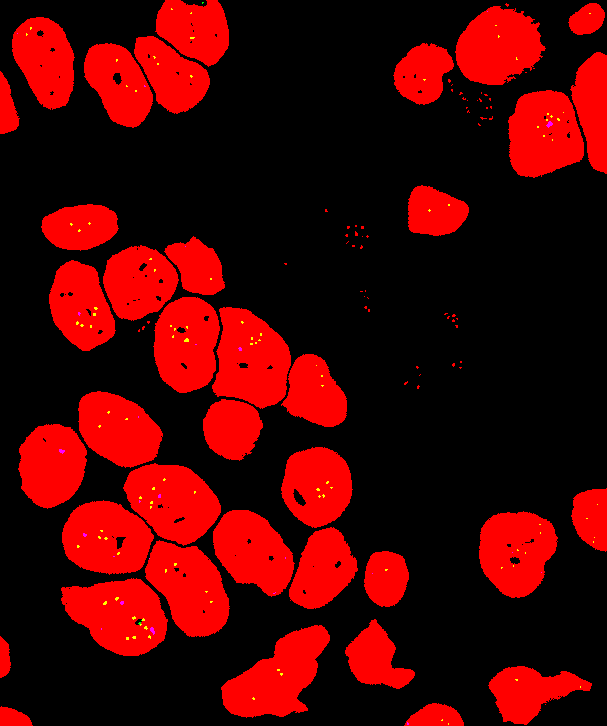
\includegraphics[width=0.5\linewidth]{data/output/fish_signal_counts/binary_masks.png}
    \caption{Initial Binary Masks for DAPI (red channel), Acridine (green channel), and FITC (blue channel).}
    \label{fig:cell_binary_masks}
\end{figure}

Figure~\ref{fig:cell_binary_masks_cleaned} shows the cleaned binary masks after morphological operations and filtering. The processed masks exhibit well-defined cell boundaries and reduced noise, facilitating accurate signal quantification. Cells that touch the image borders are marked with half-intensity in the red channel.

\begin{figure}[!htbp]
    \centering
    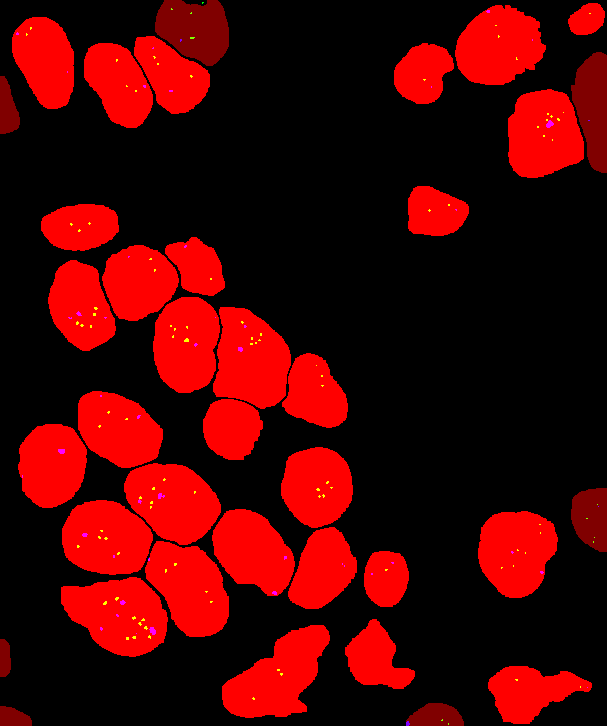
\includegraphics[width=0.5\linewidth]{data/output/fish_signal_counts/binary_masks_cleaned.png}
    \caption{Cleaned Binary Masks after Morphological Operations.}
    \label{fig:cell_binary_masks_cleaned}
\end{figure}

\subsubsection{Signal Counts and Ratios}

The pipeline successfully identified and labeled individual cells, enabling the calculation of Acridine and FITC signal counts within each cell. The program identifies 30 complete cells in the provided sample images and computes the signal counts and ratios for each cell.

Table~\ref{tab:results} shows the signal counts and ratios for a sample of cells.

\begin{table}[!htbp]
    \centering
    \caption{Signal Counts and Ratios per Cell}
    \label{tab:results}
    \begin{tabular}{|c|c|c|c|c|c|}
        \hline
        \textbf{Cell ID} & \textbf{Centroid (X, Y)} & \textbf{Area (pixels)} & \textbf{Acridine} & \textbf{FITC} & \textbf{Acridine/FITC} \\
        \hline
        1 & (586.82, 19.07) & 841 & 1 & 0 & - \\
        2 & (497.55, 45.82) & 5015 & 3 & 2 & 1.50 \\
        3 & (44.79, 60.05) & 4161 & 2 & 2 & 1.00 \\
        \ldots & \ldots & \ldots & \ldots & \ldots & \ldots \\
        30 & (530.05, 691.11) & 3332 & 2 & 1 & 2.00 \\
        \hline
    \end{tabular}
\end{table}

\newpage

\section{Application: Circuit Board Quality Assurance}

In the electronics industry, circuit board manufacturing requires stringent quality control to ensure the reliability and functionality of electronic devices. X-ray imaging is a common non-destructive technique used to inspect circuit boards for defects such as soldering issues, misalignments, and broken connections. This application focuses on analyzing an x-ray image of a circuit board to assess the quality of soldering regions, drilled holes, and connection traces.

\subsection{Methodology}

\paragraph{Input Acquisition}

The analysis begins with loading the x-ray image of the circuit board in TIFF format using the \texttt{load\_tiff\_image} function. The image has a single channel representing the intensity of the x-ray signal.

\paragraph{Preprocessing}

The x-ray image undergoes preprocessing to enhance the quality of the image:
\begin{itemize}
    \item \textbf{Noise Reduction}: Median filtering is applied to remove salt-and-pepper noise from the x-ray image. The \texttt{fix\_salt\_and\_pepper\_noise} function implements this operation by replacing pixels with extreme values \((0, 255)\) with the median of neighboring pixels.
    \item \textbf{Standardization}: It is known that soldered connections appear brighter than the rest of the traces. Soldered connections are brought to the same intensity level as the rest of the traces to treat these regions uniformly.
\end{itemize}

\paragraph{Mask Generation}

Two binary masks are generated based on the known color categories in the image:
\begin{itemize}
    \item \textbf{Holes Mask}: Produced by comparing image pixels to the value \texttt{PCBColour.HOLES}. Any pixel in the image designated as a hole location is marked as \texttt{True} (1), forming the \emph{holes mask}.
    \item \textbf{Solder Mask}: Created by combining pixels labeled as \texttt{PCBColour.SOLDER} or \texttt{PCBColour.HOLES} into one composite mask. This merged mask facilitates analysis of all solder-bearing components, including holes.
\end{itemize}

\paragraph{Morphological Opening}

To eliminate thin traces or extraneous noise, the pipeline applies a morphological opening on the solder mask via \texttt{morphological\_open}:
\begin{itemize}
    \item A kernel size of \(5 \times 5\) ensures that small spurious connections or traces are removed, effectively \emph{thickening} true solder connections and consolidating them.
    \item The resulting `thick solder' mask is then combined (logical AND) with the original solder mask to preserve only those regions that are consistently present in both masks, i.e. connectors and soldering regions, but not the PCB traces.
\end{itemize}

\paragraph{Connected Components Extraction}

Connected components labeling is performed on both the solder mask and the holes mask:
\begin{itemize}
    \item \textbf{Label Solder Regions}: The \texttt{label\_connected\_components} function detects all connected components in the `thick' solder mask, assigning a unique ID to each component.
    \item \textbf{Label Holes}: Similarly, hole regions are labeled in the holes mask. Each hole is assigned a unique ID.
\end{itemize}

\paragraph{Visualization Setup}

To produce a final color visualization of the defect analysis, an RGB image \texttt{final\_image} is initialized and populated consistently with the original x-ray image:
\begin{itemize}
    \item All background pixels default to mid-intensity grey.
    \item Pixels belonging to the solder mask are colored darker, with an additional slight intensity shift for the `thick' solder mask.
    \item Holes are colored white, ensuring high contrast against soldered areas.
\end{itemize}
This visualization enables a quick review of the pipeline's interpretation of the circuit board layout.

\paragraph{Component Inspection and Trace Integrity}

The pipeline iterates over each labeled solder component. For each component:
\begin{enumerate}
    \item \textbf{Centroid Calculation}: The centroid of the component is computed.
    \item \textbf{Sub-Region Labeling}: A label operation on the `thick' solder mask identifies further subdivisions (connectors, soldering regions) within the component.
    \item \textbf{Trace Continuity}: If the component exhibits a `thin' sub-region (i.e. a wire-like trace) that is connected (i.e. is part of the same connected component) to a single connector or soldering region, the pipeline flags a \textit{suspected broken trace}. This is done by coloring the region in red tones and appending a diagnostic message such as \texttt{Suspected broken trace touches 1 != 2 connectors}.
\end{enumerate}

\paragraph{Solder Region Assessment}

Solder sub-regions (excluding traces) are then classified based on their dimensions and shape:
\begin{enumerate}
    \item \textbf{Size Calculation}: The area of each solder sub-region is computed. If the dimensions are below a predefined threshold, the region is classified as a connector and not considered further.
    \item \textbf{Shape Determination}: For larger solder objects, we infer whether a sub-region is a circle or rectangle. This is done by measuring its minimal and maximal dimensions, and determining the fill percentage of the bounding box. If the sub-region is large, and the fill percentage is greater than 90\%, the region is classified as a rectangular soldering region; otherwise, it is considered a circular one.
    \item \textbf{Expected Mask Creation}: For each recognized soldering region shape, we generate a template mask representing an ideal solder region of the same centroid, size, and shape.
    \item \textbf{Intersection Checking}: The degree of overlap between the actual region and the expected region is computed. If they differ by more than \(5\%\), the pipeline highlights that region in red and logs a message detailing the mismatch in area and intersection.
\end{enumerate}

\paragraph{Hole Analysis}

Each solder sub-region should contain exactly one hole. After identifying the hole(s) within a solder region:
\begin{itemize}
    \item \textbf{Hole Count}: The pipeline checks how many hole labels intersect with the sub-region. If this count is not exactly one, a warning is generated indicating an anomaly (e.g., missing hole, extra holes).
    \item \textbf{Hole Dimensions and Position}: Hole centroids and dimensions are evaluated similarly to solder regions. The pipeline creates a corresponding \emph{expected hole} mask, verifying shape and size. Deviations in centroid location or dimensions produce warning messages and these discrepancies are highlighted visually in the final image.
\end{itemize}

\paragraph{Final Output}

Upon completing the inspections, the final image is saved, reflecting all colored overlays indicating solder coverage, holes, and flagged defects.

\subsection{Running the Analysis}

Terminal command to run the analysis:

\begin{lstlisting}[language=bash]
$ python python/main.py circuit-board-qa \
    <input_path>
\end{lstlisting}

Here, the \texttt{input\_path} is the file path to the x-ray image of the circuit board. In this analysis, we processed the provided sample image:

\begin{lstlisting}[language=bash]
$ python python/main.py circuit-board-qa \
    "data/input/pcb-xray.tif"
\end{lstlisting}

\subsection{Results}

\subsubsection{Visualizations of Intermediate Steps}

Figure~\ref{fig:image_raw} shows the raw x-ray image of the circuit board. The image contains salt-and-pepper noise, which can obscure internal structures and components.

\begin{figure}[!htbp]
    \centering
    \includegraphics[width=0.5\linewidth]{data/output/circuit_board_qa/image_raw.png}
    \caption{Raw X-ray Image of the Circuit Board.}
    \label{fig:image_raw}
\end{figure}

Figure~\ref{fig:image_denoised} shows the denoised x-ray image of the circuit board after applying the median filter. The image is now clearer, with salt-and-pepper noise removed, enhancing the visibility of internal structures.

\begin{figure}[!htbp]
    \centering
    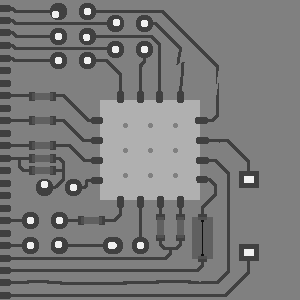
\includegraphics[width=0.5\linewidth]{data/output/circuit_board_qa/image_denoised.png}
    \caption{Denoised X-ray Image of the Circuit Board.}
    \label{fig:image_denoised}
\end{figure}

Figure~\ref{fig:final_image} shows the final image with detected defects highlighted in red. The soldering regions, drilled holes, and connection traces are clearly visible, with broken connections, wrong-sized soldering regions, and misaligned holes flagged for inspection.

\begin{figure}[!htbp]
    \centering
    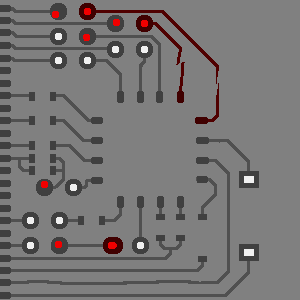
\includegraphics[width=0.5\linewidth]{data/output/circuit_board_qa/final_image.png}
    \caption{Cleaned Binary Masks after Morphological Operations.}
    \label{fig:final_image}
\end{figure}

\subsubsection{List of Detected Defects}

The complete list of defects detected in the circuit board image is printed in the terminal output. For each defect, the pipeline provides the defect ID, location (X, Y), and a description of the issue. We provide a summary of the defects in Table~\ref{tab:defects}.

\begin{table}[!htbp]
    \centering
    \caption{Detected Defects in the Circuit Board}
    \label{tab:defects}
    \begin{tabular}{|c|c|p{0.6\linewidth}|}
        \hline
        \textbf{Defect ID} & \textbf{Location (X, Y)} & \textbf{Description} \\
        \hline
        1 & (58.00, 11.00) & Round soldering region has hole at centroid: (14.0, 55.0), expected: (11.0, 58.0) \\
        2 & (141.45, 23.79) & Suspected broken trace touches 1 != 2 connectors \\
        3 & (115.00, 23.00) & Round soldering region has hole at centroid: (22.0, 116.0), expected: (23.0, 115.0) \\
        4 & (155.07, 30.42) & Suspected broken trace touches 1 != 2 connectors \\
        5 & (87.00, 36.00) & Round soldering region has hole at centroid: (36.95, 86.07), expected: (36.0, 87.0) \\
        6 & (180.70, 85.88) & Suspected broken trace touches 1 != 2 connectors \\
        7 & (209.50, 112.46) & Suspected broken trace touches 1 != 2 connectors \\
        8 & (44.00, 187.00) & Round soldering region has hole at centroid: (184.0, 44.0), expected: (187.0, 44.0) \\
        9 & (58.97, 245.02) & Round soldering region has hole at centroid: (244.0, 58.0), expected: (245.02, 58.97) \\
        10 & (112.50, 245.00) & Round soldering region, area: 292, expected: 242, intersection: 242 \\
        11 & (112.50, 245.00) & Round soldering region has hole at centroid: (245.0, 111.75), expected: (245.0, 112.5) \\
        12 & (111.75, 245.00) & Round soldering region has hole with dimensions: (7, 9), expected: (7, 7) \\
        13 & (111.75, 245.00) & Round hole, area: 55, expected: 44, intersection: 44 \\
        \hline
    \end{tabular}
\end{table}

\newpage

\section{Application: Filled Bottles}

% Digital image processing is a field that involves the analysis and manipulation of digital images using algorithms to extract information or enhance image quality. In the context of industrial automation, such as bottle filling detection, this field is crucial for quality control and efficiency. Key concepts include image segmentation, edge detection, and feature extraction, all of which are instrumental in identifying specific regions or characteristics within an image.

% In this task, we leverage grayscale intensity levels, edge detection algorithms, and geometric analysis to determine the liquid level in the bottles. The liquid level can be defined as the boundary between the high-intensity region (bottle body) and the low-intensity region (air above the liquid). Robustness to varying lighting conditions and image acquisition inconsistencies is achieved by normalizing image brightness and employing adaptive thresholding techniques.

% Theoretical challenges addressed in this context include:
% \begin{itemize}
%     \item Variations in lighting conditions due to production environment differences.
%     \item Variability in camera positions and zoom levels that affect the perceived dimensions of bottles.
%     \item Potential occlusions or artifacts caused by reflections, labels, or other bottle features.
% \end{itemize}

\subsection{Methodology}

% The algorithm for detecting improperly filled bottles is structured as follows:

% \begin{enumerate}
%     \item \textbf{Preprocessing:} The input image is converted to grayscale, and histogram equalization is applied to normalize brightness. This step ensures uniform lighting conditions across the production line.
%     \item \textbf{Edge Detection:} Canny edge detection is employed to identify the contours of the bottle. The edges are used to locate key structural points, such as the neck, shoulder, and base of the bottle.
%     \item \textbf{Region of Interest (ROI) Extraction:} Based on the detected edges, the region between the neck and shoulder of the bottle is identified as the area of interest.
%     \item \textbf{Liquid Level Detection:} Adaptive thresholding is applied within the ROI to distinguish between the liquid region and the air region. The midpoint between the neck and shoulder is calculated, and the detected liquid level is compared to this threshold.
%     \item \textbf{Decision Making:} If the liquid level is below the calculated midpoint, the bottle is flagged as improperly filled.
% \end{enumerate}

% Assumptions made in this methodology include:
% \begin{itemize}
%     \item The bottle geometry (neck and shoulder) is consistent across all samples.
%     \item Images are free from motion blur due to the use of flash illumination.
%     \item The liquid is optically distinguishable from the bottle material.
% \end{itemize}

% These assumptions, while simplifying the implementation, may limit the robustness of the solution in highly variable production environments. Additional calibration steps or machine learning-based feature extraction methods can be integrated to address these challenges.

\subsection{Running the Analysis}

Terminal command to run the analysis:

\begin{lstlisting}[language=bash]
$ python python/main.py filled-bottles \
    <input_path>
\end{lstlisting}

Here, the \texttt{input\_path} is the file path to the image of the filled bottles. In this analysis, we processed the provided sample image:

\begin{lstlisting}[language=bash]
$ python python/main.py filled-bottles \
    data/input/Bottles.tif
\end{lstlisting}

\subsection{Results}

\subsubsection{Visualizations of Intermediate Steps}

The intermediate steps of the analysis are visualized in the output images. Figure~\ref{fig:bottle_raw} shows the raw image of the filled bottles. The image contains five bottles with varying liquid levels. Two bottles sit on the border of the image, and were not analyzed. Out of the remaining three bottles, the middle bottle is underfilled.

\begin{figure}[!htbp]
    \centering
    \includegraphics[width=0.5\linewidth]{data/output/filled_bottles/image_raw.png}
    \caption{Raw Image of Filled Bottles.}
    \label{fig:bottle_raw}
\end{figure}

The processed image with detected liquid levels is shown in Figure~\ref{fig:bottle_processed}. The background is black, the liquid level is marked in grey, and the air region is white. The neck and shoulder regions are displayed as black horizontal lines. It is evident that the middle bottle is underfilled, as the liquid level is below the midpoint between the neck and shoulders.

\begin{figure}[!htbp]
    \centering
    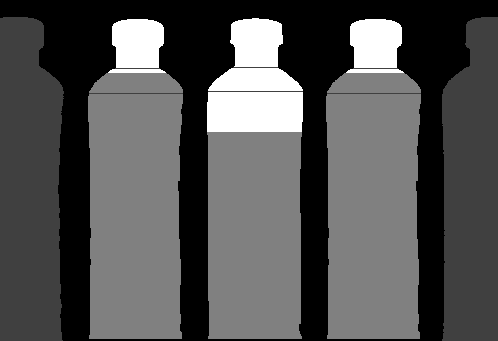
\includegraphics[width=0.5\linewidth]{data/output/filled_bottles/final_image.png}
    \caption{Processed Image with Detected Liquid Levels.}
    \label{fig:bottle_processed}
\end{figure}

\subsubsection{Liquid Level in Provided Sample Image}

The image analysis script prints the results of the liquid level detection for each bottle in the sample image. Table~\ref{tab:bottle_results} shows the results for the provided sample image.

\begin{table}[!htbp]
    \centering
    \caption{Liquid Level Detection Results for Sample Bottles}
    \label{tab:bottle_results}
    \begin{tabular}{|c|c|c|c|c|}
        \hline
        \textbf{Bottle ID} & \textbf{Centroid (X, Y)} & \textbf{Liquid Level} & \textbf{Neck-Shoulder Range} & \textbf{Filled} \\
        \hline
        1 & (254.23, 190.84) & 132 & 67-92 & False \\
        2 & (134.80, 190.69) & 73 & 68-94 & True \\
        3 & (372.80, 190.69) & 73 & 68-94 & True \\
        \hline
    \end{tabular}
\end{table}

The method was tested on a synthetic dataset of hand-crafted images, simulating various liquid levels in bottles. The results were omitted for brevity but demonstrated the algorithm's robustness in detecting improperly filled bottles at different liquid levels and lighting conditions.

\end{document}
